%-------------------------
%big-picture
%(c) H.Buchmann FHNW 2008
%$Id$
%export TEXINPUTS=${HOME}/fhnw/edu/tinL/config/latex:${HOME}/fhnw/edu/config//:
%-------------------------
\documentclass{beamer}
\usepackage{latex/beamer}
%---------------------
%local defines
%(c) H.Buchmann FHNW 2009
%$Id$
%---------------------
\def \target {\raspberry\xspace}
\def \host {{\em Host \xspace}}

\title[Setup]{Setup}
\begin{document}

\frame{\titlepage}

\begin{frame}{Ziel}{Verbindung: Host-Target}
 \begin{description}
  \item[Host] \linux 
  \begin{itemize}
   \item als virtuelle Maschine
   \item native
   \item Distribution: Ubuntu
  \end{itemize}
 \item[Target]
  \begin{itemize}
   \item \beaglebone per USB
   \begin{itemize}
    \item Speicher: USB Stick 
	\item Serielle Schnittstelle \cod{/dev/ttyACM0}
	\item Ethernet
   \end{itemize}
  \end{itemize}
  \item[Verbindung]
  \begin{itemize}
   \item \cod{ping}
   \item \cod{ssh}
  \end{itemize}
 \end{description}
\end{frame}

\begin{frame}{Terminologie}
 \begin{description}[Target]
  \item[Host] der Entwicklungsrechner Notebook
  \item[Target] \beaglebone
 \end{description}
\end{frame}

%\section{Image}
%%-------------------------
%big-picture
%(c) H.Buchmann FHNW 2008
%$Id$
%export TEXINPUTS=${HOME}/fhnw/edu/:${HOME}/fhnw/edu/tinL/config/latex:${HOME}/fhnw/edu/config//:
%-------------------------
\documentclass{beamer}
\usepackage{latex/beamer}
%---------------------
%local defines
%(c) H.Buchmann FHNW 2009
%$Id$
%---------------------
\def \target {\raspberry\xspace}
\def \host {{\em Host \xspace}}


\title{Image auf SD Karte}
\begin{document}

\newcommand{\distro}{sd-2016-09-28.img.gz}

\frame{\titlepage}

\begin{frame}{Ziel}{Image auf SD-Karte}
 \begin{itemize}
  \item Wie startet ein Rechner
  \begin{itemize}
   \item booten
  \end{itemize}
  \item Partitionen
  \begin{itemize}
   \item alles ist ein File
  \end{itemize}
  \item die serielle Schnittstelle via USB
  \begin{itemize}
   \item der erste Kontakt mit dem \target
  \end{itemize}
  \item Image
  \begin{itemize}
   \item per USB am lokalen Netz \host - \targetS
   \item per Wi-Fi am Internet
  \end{itemize}
 \end{itemize}
\end{frame}

%-------------------------
%minimal-unix
%(c) H.Buchmann FHNW 2014
%export TEXINPUTS=.:${HOME}/fhnw/edu/:${HOME}/fhnw/edu/tinL/config/latex:${HOME}/fhnw/edu/config//:
%-------------------------
\documentclass{beamer}
\usepackage{latex/beamer}
%---------------------
%local defines
%(c) H.Buchmann FHNW 2009
%$Id$
%---------------------
\def \target {\raspberry\xspace}
\def \host {{\em Host \xspace}}

\input{/home/buchmann/latex/dirtree/dirtree.tex}

\usepackage[absolute]{textpos}
\setlength{\TPHorizModule}{1mm}
\setlength{\TPVertModule}{1mm}

\begin{document}

\newcommand{\md}{\cod{md-bbb-{\em version}.img}}
\newcommand{\mdev}{\cod{md-bbb-devel-{\em version}.tar.gz}}
\title[Boot]{Boot\\die verschiedenen M�glichkeiten}

\frame{\titlepage}

\begin{frame}{\target} {Die Boot Devices}
  \begin{description}
   \item[SPI0] {\bf S}erial {\bf P}eripheral {\bf I}nterface
   \item[MMC1] die eingebaute SD-Card
   \item[MMC0] die externe SD-Card
   \item[UART0] die serielle Schnittstelle
   \item[USB0] USB Schnittstelle
  \end{description}
\end{frame}

\begin{frame}{\target}{zwei M�glichkeiten}
\begin{columns}
\begin{column}{0.5\textwidth}
 \begin{itemize}
  \item die normale:
   \begin{itemize}
    \item \cod{MMC1}, \cod{MMC0}, \cod{UART0}, \cod{USB0}
   \end{itemize}
   \item Boot Switch
   \begin{itemize}
    \item \cod{SPI0}, \cod{MMC0}, \cod{USB0}, \cod{UART0}
   \end{itemize}
 \end{itemize}
\end{column}
\begin{column}{0.5\textwidth}
 \includegraphics[width=0.75\textwidth]{boot-switch.pdf}
\end{column}
\end{columns} 
\end{frame}

\end{document}

\section{Partitionen}
\begin{frame}{Partition}
 \begin{itemize}
  \item Träger von Filesystemen
  \item Aufbau
  \begin{itemize}
   \item MBR: Master Boot Record
  \end{itemize}
  \item Herstellung
 \end{itemize}
 \remark{Alles ist ein File  {\em stream of bits}}
\end{frame}

\subsection{Massenspeicher}
\begin{frame}{Massenspeicher}{non volatile}
 \begin{block}{Arten}
  \begin{itemize}
   \item mechanische Festplatten
   \item SSD Karten
   \item SD-Karten
   \item Flash
   \item ...
  \end{itemize}
 \end{block}
 \begin{block}{Typisch}
  \begin{itemize}
   \item Zugriff relativ langsam
   \item Blockorientiert 
   \begin{itemize}
    \item Mehrere Bits/Bytespro Zugriff
   \end{itemize}
  \end{itemize}
 \end{block}
\end{frame}


\begin{frame}{Partitionen Termiologie \linux}{Träger von Filesystemen}
  \begin{itemize}
   \item Massenspeicher
   \begin{itemize}
   \item \cod{/dev/sd{\em X}}, \cod{{\em X}=a,b,c ...}
   \end{itemize} 
   \item Partitionen 
   \begin{itemize}
     \item \cod{/dev/sd{\em X}{\em N}} \cod{{\em N}=1,2,3 ...} 
   \end{itemize} 
  \end{itemize}
  \begin{block}{\Huge Vorsicht}
   \begin{itemize}
    \item Festplatte vom \host ist auch ein \cod{/dev/sd{\em X}}
   \end{itemize}
  \end{block}
\end{frame} 


\begin{frame}[fragile]{Massenspeicher}{Blocks/Sektoren}
\begin{lstlisting}
 typedef unsigned char Sector[512]; 
 Sector MassStorage[N];
\end{lstlisting}
\remark{Ein langer Array von Sektoren}
\begin{center}
\includegraphics[width=0.875\textwidth]{array-of-sector.jpg}
\end{center}
\end{frame}

\begin{frame}[fragile]{Der Befehl \cod{dd}}{Vorsicht}
\begin{lstlisting}[language=bash]
dd if=/dev/sdX count=1|hexdump -C        
  # first sector to stdout
dd if=/dev/sdX skip=1 count=1|hexdump -C 
  # second sector to stdout
dd if=/dev/sdX of=mbr.bin count=1        
  # copy sector to mbr.bin
\end{lstlisting}
  \begin{block}{\Huge Vorsicht}
   \begin{itemize}
    \item Festplatte vom \host ist auch ein \cod{/dev/sd{\em X}}
   \end{itemize}
  \end{block}

\end{frame}

\subsection{MBR}
\begin{frame}[fragile]{MBR: Master Boot Record}{Verzeichnis der Partionen}
\begin{lstlisting}[language=bash]
dd if=/dev/mmcblk0 count=1|hexdump -C
\end{lstlisting}
{\scriptsize
\begin{verbatim}
00000000  00 00 00 00 00 00 00 00  00 00 00 00 00 00 00 00  |................|
*
000001b0  00 00 00 00 00 00 00 00  ba 23 8e d6 00 00 00 00  |.........#......|
000001c0  01 20 0b 03 10 1f 00 08  00 00 00 00 04 00 00 00  |. ..............|
000001d0  01 20 83 03 50 df 00 08  04 00 00 70 71 00 00 00  |. ..P......pq...|
000001e0  00 00 00 00 00 00 00 00  00 00 00 00 00 00 00 00  |................|
000001f0  00 00 00 00 00 00 00 00  00 00 00 00 00 00 55 aa  |..............U.|
00000200
\end{verbatim}
}

{\scriptsize\url{technet.microsoft.com/en-us/library/cc976786.aspx}}

\end{frame}


\section{Serielle Schnittstelle}
\begin{frame}{USB-Serial}
\begin{columns}
\begin{column}{0.5\textwidth}
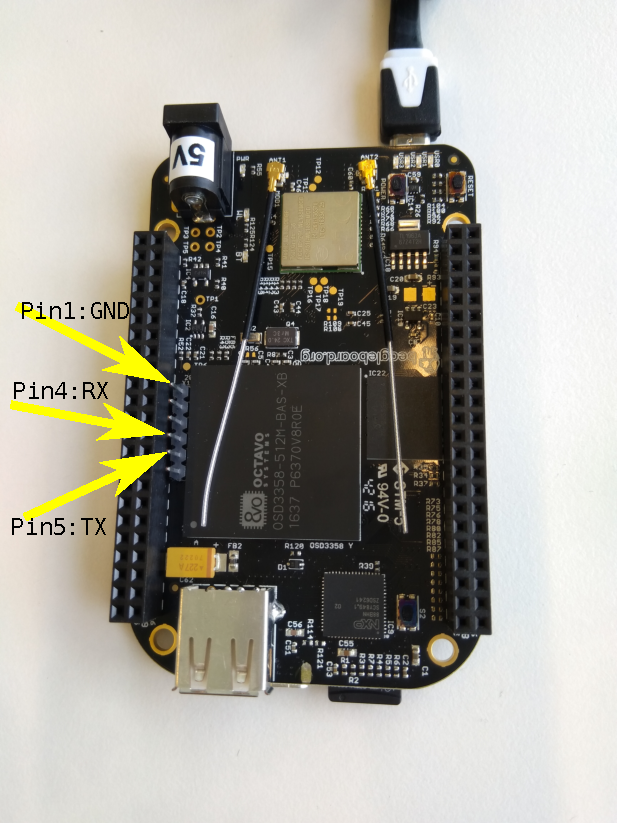
\includegraphics[height=0.825\textheight]{pin.pdf}
\end{column}
\begin{column}{0.5\textwidth}
\begin{block}{Cable}
\vspace{5mm}
\begin{tabular}{c|c}
Color & Signal\\
\hline
BLACK & GND\\
GREEN & TX\\
WHITE & RX
\end{tabular}
\end{block}
\end{column}
\end{columns}
\end{frame}



\section{SD Karte}
\begin{frame}{Initiale SD-Karte}{Herstellung}
 \begin{itemize}
  \item das Image:
  \begin{itemize}
   \item \href{https://drive.switch.ch/index.php/s/A6H382zEGDrgfAL}{sd-2020-03-04.img.xz}
  \end{itemize}
  \item auf SD-Karte
  \begin{itemize}
   \item \cod{xz -d -c sd-2020-03-04.img.xz | sudo dd of=/dev/sdX}
   \begin{remarks}
   \item {\Huge Vorsicht} bei \cod{/dev/sdX}
   \item File \cod{sd-2020-03-04.img.xz} im \href{https://drive.switch.ch/index.php/s/A6H382zEGDrgfAL}
                      {\color{red}$\to$Verzeichnis}
   \end{remarks}
  \end{itemize}
 \end{itemize}
\end{frame}

\begin{frame}[fragile]{2 Partitionen}{gemacht mit \cod{fdisk -l /dev/sdX}}
{
\footnotesize
\begin{verbatim}
Disk /dev/sda: 14.5 GiB, 15552479232 bytes, 30375936 sectors
Disk model: STORAGE DEVICE  
Units: sectors of 1 * 512 = 512 bytes
Sector size (logical/physical): 512 bytes / 512 bytes
I/O size (minimum/optimal): 512 bytes / 512 bytes
Disklabel type: dos
Disk identifier: 0x00000000

Device     Boot Start    End Sectors  Size Id Type
/dev/sda1  *     2048  34815   32768   16M  b W95 FAT32
/dev/sda2       34816 559103  524288  256M 83 Linux
\end{verbatim}
}
\begin{description}
 \item[p1] Boot Partition
 \item[p2] Root Filesystem das Linux
\end{description}
\end{frame}

%\subsection{Distribution}
%\begin{frame}[fragile]{Alles ist ein File}{und umgekehrt}
%\begin{itemize}
% \item Der File \cod{\distro}
% ist das Bild einer ganzen SD-Karte
% \item Mache SD-Karte
% \begin{itemize}
%  \item Kopiere {\tiny\url{sourceforge.net/projects/fhnw-tinl/files/{\distro}/download}} 
%  \item entzippe
%  \item kopiere
%  \begin{lstlisting}
%dd if=distro.img of=/dev/sd-card
%  \end{lstlisting}
%  \cod{sd-card} typ \cod{mmcblk\em{N}} $N=0|1 ..$
% \end{itemize}
% \remark{Alles mit {\em pipes}}
% 
%\end{itemize}
%
%\end{frame}

\end{document}



\begin{frame}{USB: Linux Foundation Multifunction Composite Gadget}
             {der Befehl \cod{lsusb} auf dem \host}
  \begin{itemize}
   \item \cod{lsusb} f�r den �berblick
   \item \cod{lsusb -d 1d6b:0104} der \beaglebone
   \begin{itemize}
    \item \cod{lsusb -v -d 1d6b:0104} was \beaglebone alles kann
   \end{itemize} 
  \end{itemize}
\end{frame}

\section{Mass Storage}
\begin{frame}{Mass Storage}{\beaglebone als USB Stick} 
 \begin{itemize}
  \item der Befehl \cod{ls}
  \begin{itemize}
   \item \cod{ls {\em mount-point}}
   \item wo ist der \cod{{\em mount-point}}
  \end{itemize}
 \end{itemize}
\end{frame}

\section{RS232}
\begin{frame}{Communications device class CDC}{Terminal Programm \cod{minicom}}
 \begin{itemize}
  \item \cod{minicom -D /dev/tty{\em XYZ}} \cod{\em XYZ} typ. \cod{ACM0}
  \item einfache Bedienung
  \begin{itemize} 
   \item \cod{CTRL-A} Z for help
   \item \cod{CTRL-A} O Configuration
   \begin{itemize}
    \item Baudrate 115200
    \item no HW Handshake
    \item no SW Handshake
   \end{itemize}
   \item \cod{ESC} escape Schritt zurück
  \end{itemize}
 \end{itemize}
\end{frame}

%-------------------------
%big-picture
%(c) H.Buchmann FHNW 2008
%$Id$
%export TEXINPUTS=${HOME}/fhnw/edu/:${HOME}/fhnw/edu/tinL/config/latex:${HOME}/fhnw/edu/config//:
%-------------------------
\documentclass{beamer}
\usepackage{latex/beamer}
%---------------------
%local defines
%(c) H.Buchmann FHNW 2009
%$Id$
%---------------------
\def \target {\raspberry\xspace}
\def \host {{\em Host \xspace}}

\input{/home/buchmann/latex/dirtree/dirtree.tex}

\title[Netzwerk]{Netzwerk}
\begin{document}

\frame{\titlepage}

\begin{frame}{Ziel}{\target am Schulnetz}
 \begin{itemize}
  \item Verschiedene Netze
  \begin{itemize}
   \item {\em Schulnetz} passwortgesch�tzt
   \item {\em lokales Netz} \host{} \target 
  \end{itemize}
  \item Gesucht
  \begin{itemize}
   \item Verbindung {\em Schulnetz} $\leftrightarrow$ {\em lokales Netz}
  \end{itemize}
  \item Wichtiger Begriff
  \begin{description}
   \item[Proxy] Stellvertreter
  \end{description}
  \item Was wir m�chten
  \begin{itemize}
   \item \cod{HTTP} auf \target
   \item \cod{apt-get ...}
  \end{itemize}
 \end{itemize}
\end{frame}

\begin{frame}{Zwei Netze}{zwei Rechner}
 \begin{center}
 \includegraphics[width=0.875\textwidth]{two-networks.png}
 \end{center}
 \begin{itemize}
  \item Netze
  \begin{description}[LokalesNetz (LN)]
  \item[Schulnetz   (SN)] {\em mit} Verbindung zum Internet
  \item[LokalesNetz (LN)] {\em ohne} Verbindung zum Internet
  \end{description}
  \item Rechner
  \begin{description}[\target(BBB)]
   \item[Workstation(WS)] am SN und LN
   \item[\target(BBB)] am LN  
  \end{description}
 \end{itemize}
\end{frame}

\section{HTTT Proxy}

\begin{frame}{Proxy}{Stellvertreter}
  \begin{center}
 \includegraphics[width=0.875\textwidth]{proxy.pdf}
 \end{center}
 \begin{itemize}
  \item Server auf \host
  \item reicht die \cod{http} {\em requests/responses} weiter
 \end{itemize}

\end{frame}

\begin{frame}{Test mit \cod{curl}}{\url{curl.haxx.se/}}
  \begin{itemize}
   \item \cod{curl address}
   \begin{itemize}
    \item \cod{curl fhnw.ch}
   \end{itemize}
  \end{itemize}
\end{frame}

\begin{frame}{Proxy Server}{drei Vorschl�ge}
 \begin{itemize}
  \item \cod{tinyproxy}
  \vspace{-5mm}
  \begin{quote}
  lightweight http(s) proxy daemon
  \end{quote}
  \begin{itemize}
   \item {\scriptsize\url{tinyproxy.github.io}}
  \end{itemize}
  \item \cod{polipo}
   \vspace{-5mm}
   \begin{quote} 
   is a lightweight caching and forwarding web proxy server
   \end{quote}
%   \vspace{-5mm}
   \begin{itemize}
    \item {\scriptsize\url{www.pps.univ-paris-diderot.fr/~jch/software/polipo/}}
   \end{itemize}
  \item \cod{squid}
   \vspace{-5mm}
   \begin{quote} 
   is a caching proxy for the Web supporting
   \end{quote}
   \begin{itemize}
     \item {\scriptsize\url[http]{www.squid-cache.org/}}
   \end{itemize}
 \end{itemize}
\end{frame}


\begin{frame}{\cod{tinyproxy}}{direkter Aufruf}
 \begin{description}[\target]
  \item[\host] Skript Server
  \begin{itemize}
   \item \cod{./tools/tinyproxy.sh}
  \end{itemize}
  \item[\target] Client
  \begin{itemize}
   \item \cod{curl --proxy http://192.168.7.1:8888  \textbackslash\\ www.google.ch}
  \end{itemize}
 \end{description}
 \remark{Wie steht es mit \cod{https}}
\end{frame}

\begin{frame}{\target}{\cod{apt-get}}
 \begin{itemize}
  \item Konfiguration \targetS
  \begin{itemize}
   \item File \cod{/etc/apt/apt.conf.d/05proxy}
   \begin{itemize}
    \item \cod{Acquire::http::proxy "{}http://192.168.7.1:8888"{};}
   \end{itemize}
  \end{itemize}
  \item Test
  \begin{itemize}
   \item \cod{apt-get update}
   \item \cod{apt-get install sshfs}
  \end{itemize}
 \end{itemize}
\end{frame}


\section{SSH}
\begin{frame}{\target}{SSH TODO}
% \begin{itemize}
%  \item \cod{ssh -D{\em port} user@host}
%  \item \cod{curl --proxy socks5h localhost:{\em port} {\em http:address}}
%  \item \cod{atp-get} funktioniert nicht
%  \begin{itemize}
%   \item File \cod{apt.conf.d/05proxy} 
%    \begin{itemize}
%     \item \cod{Acquire::http::proxy "{}socks4a://localhost:8123"{};}
%	 \item[] oder ??
%	 \item \cod{Acquire::socks::proxy "{}socks4a://localhost:8123"{};}
%	 \item port=8123
%    \end{itemize}
%  \end{itemize}
% \end{itemize}
\end{frame}

\section{Forwarding}
\begin{frame}{Forwarding}{\host ist ein router}
 \begin{center}
  \includegraphics[width=0.875\textwidth]{router.pdf}
 \end{center}
 \begin{itemize}
  \item alle IP Protokolle 
  \item NAT Network Address Translation
 \end{itemize}
\end{frame}

\begin{frame}[fragile]{Konfiguration}
 \begin{description}[\target]
  \item[\host] \cod{tools/forwarding.sh}
  \item[\target] Setze gateway
  \begin{lstlisting}[language=bash]
  route add default gw host-ip usb0
  \end{lstlisting}
  \item Setze DNS Server
  \begin{itemize}
   \item \cod{cp config/resolv.conf /etc/resolv.conf}
  \end{itemize}
  einfach aber nicht universell
 \end{description}
\end{frame}

\section{Aufgaben}
\subsection{Proxy}

\begin{frame}{Aufgaben}{Proxy}
 \begin{itemize}
  \item Installiere Proxy
  \item Teste Proxy 
  \item Was wird auf den lokalen Netz �bertragen 
  \begin{itemize}
   \item \cod{wireshark}
  \end{itemize}
  \item Setze \cod{apt-get} \& Co. so auf, dass \target per Internet/Proxy funktioniert 
 \end{itemize}
\end{frame}

\subsection{Forwarding}

\begin{frame}{Aufgaben}{Forwarding}
 \begin{itemize}
  \item Setze \host auf
  \item Setze \target auf
  \item Teste mit \cod{ping}
  \item Test mit \cod{apt-get}
 \end{itemize}
\end{frame}

\end{document}




\end{document}

